\subsection{Ecuación de calor}

Los programas y resultados del problema 1a y 1b se encuentran en la carpeta \folder{Problema\_1}. Cada inciso tiene su propia carpeta llamadas \folder{Problema\_1a} y\folder{Problema\_1b}.
\subsubsection{Problema 1a}
\begin{itemize}
    \item \textbf{Resolver la ecuación de calor considerando \{Q = 3, K = 5, u\textsubscript{0} = 10, u\textsubscript{n} = 20, n = 4, L = 1\}, L es la longitud de la barra.}

          Para este caso se puede visualizar el sistema de ecuaciones, el cual es el siguiente:

          \begin{equation}
              \begin{pmatrix}
                  2  & -1 & 0  \\
                  -1 & 2  & -1 \\
                  0  & -1 & 2
              \end{pmatrix}
              \begin{pmatrix}
                  u_1 \\
                  u_2 \\
                  u_3
              \end{pmatrix}
              =\begin{pmatrix}
                  10.037500 \\
                  0.037500  \\
                  20.037500
              \end{pmatrix}
              \label{eq:heat_matrix_problem1a}
          \end{equation}

          La solución del sistema \ref{eq:heat_matrix_problem1a} es el siguiente:

          \begin{equation}
              \begin{pmatrix}
                  u_0 \\
                  u_1 \\
                  u_2 \\
                  u_3 \\
                  u_4
              \end{pmatrix}    =
              \begin{pmatrix}
                  10        \\
                  12.556250 \\
                  15.075000 \\
                  17.556250 \\
                  20
              \end{pmatrix}
              \label{eq:problem1a_solution}
          \end{equation}


    \item \textbf{Resolver la ecuación de calor considerando \{Q = 3, K = 5, u\textsubscript{0} = 10, u\textsubscript{n} = 20, n = 100, L = 1\}.}

          El sistema de ecuaciones para el problema es el siguiente:

          \begin{equation}
              \begin{pmatrix}
                  2      & -1     & 0      & 0      & \cdots & 0      \\
                  -1     & 2      & -1     & 0      & \cdots & 0      \\
                  0      & -1     & 2      & -1     & \cdots & 0      \\
                  0      & 0      & -1     & 2      & \cdots & 0      \\
                  \vdots & \vdots & \vdots & \vdots & \vdots & \vdots \\
                  0      & 0      & 0      & -1     & 2      & -1     \\
                  0      & 0      & 0      & 0      & -1     & 2
              \end{pmatrix}
              \begin{pmatrix}
                  u_0    \\
                  u_1    \\
                  u_2    \\
                  u_3    \\
                  \vdots \\
                  u_{98} \\
                  u_{99}
              \end{pmatrix}
              =\begin{pmatrix}
                  10.000060 \\
                  0.000060  \\
                  0.000060  \\
                  0.000060  \\
                  0.000060  \\
                  0.000060  \\
                  20.000060 \\
              \end{pmatrix}
              \label{eq:heat_matrix_problem1b}
          \end{equation}

          La solución del sistema de ecuaciones \ref{eq:heat_matrix_problem1b} se encuentra en el archivo \file{Solution\_100.txt}.
\end{itemize}
\subsubsection{Problema 1b}

\textbf{Graficar la variación de temperatura u del nodo central contra el número de elementos n $\in$ \{10, 30, 50, 70, 100\} que equivale a n + 1 nodos.}

Para este problema se creo un ciclo que repetirá el proceso del problema 1a. En este ciclo, el valor de $n$ cambiará para obtener la solución del problema. Los archivos que contienen el resultado del nodo central y  anterior al central de cada iteración son \file{results\_1.csv} y \file{results\_2.csv} respectivamente. Se creo un programa en python, el cual lee el archivo de resultados y realiza las gráficas \ref{fig:heat_results_1} y \ref{fig:heat_results_2}.

\begin{center}
    \begin{minipage}{0.45\linewidth}
        \begin{figure}[H]
            \centering
            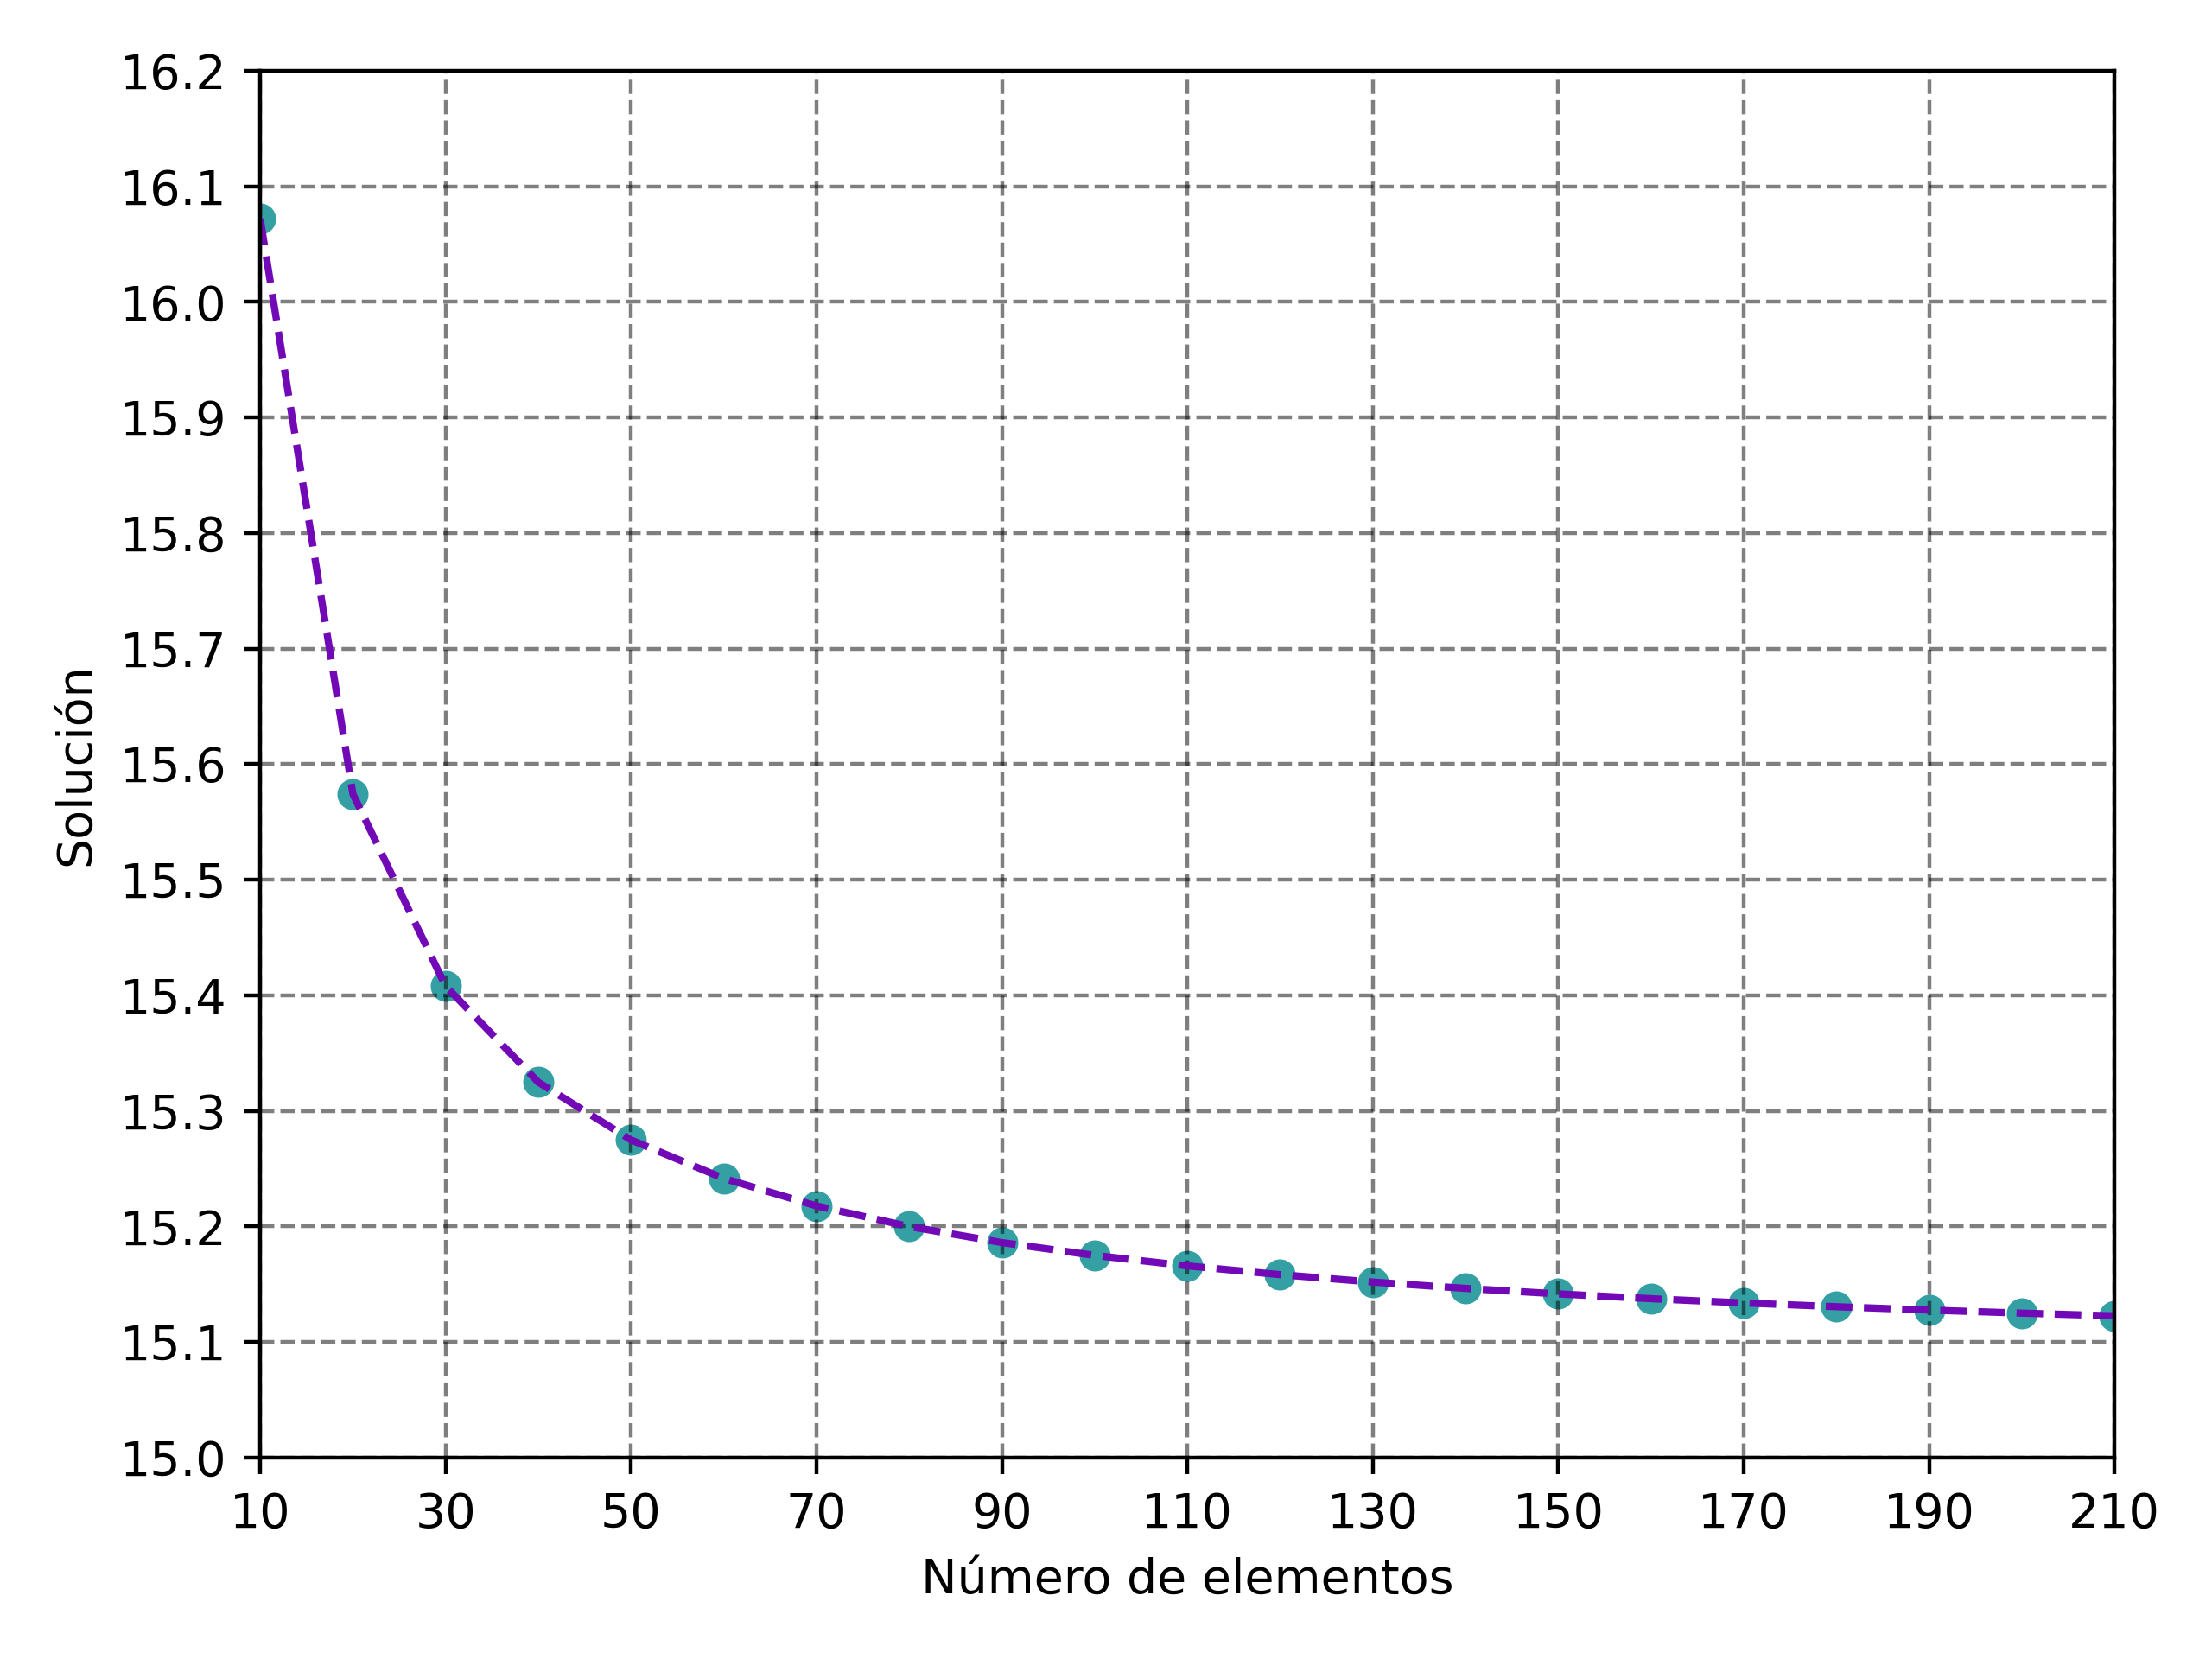
\includegraphics[width=7.5cm]{Graphics/heat_results_1.png}
            \caption{Resultado del nodo central ($\frac{n}{2}$) para cada valor de n.}
            \label{fig:heat_results_1}
        \end{figure}
    \end{minipage}
    \hspace{0.5cm}
    \begin{minipage}{0.45\linewidth}
        \begin{figure}[H]
            \centering
            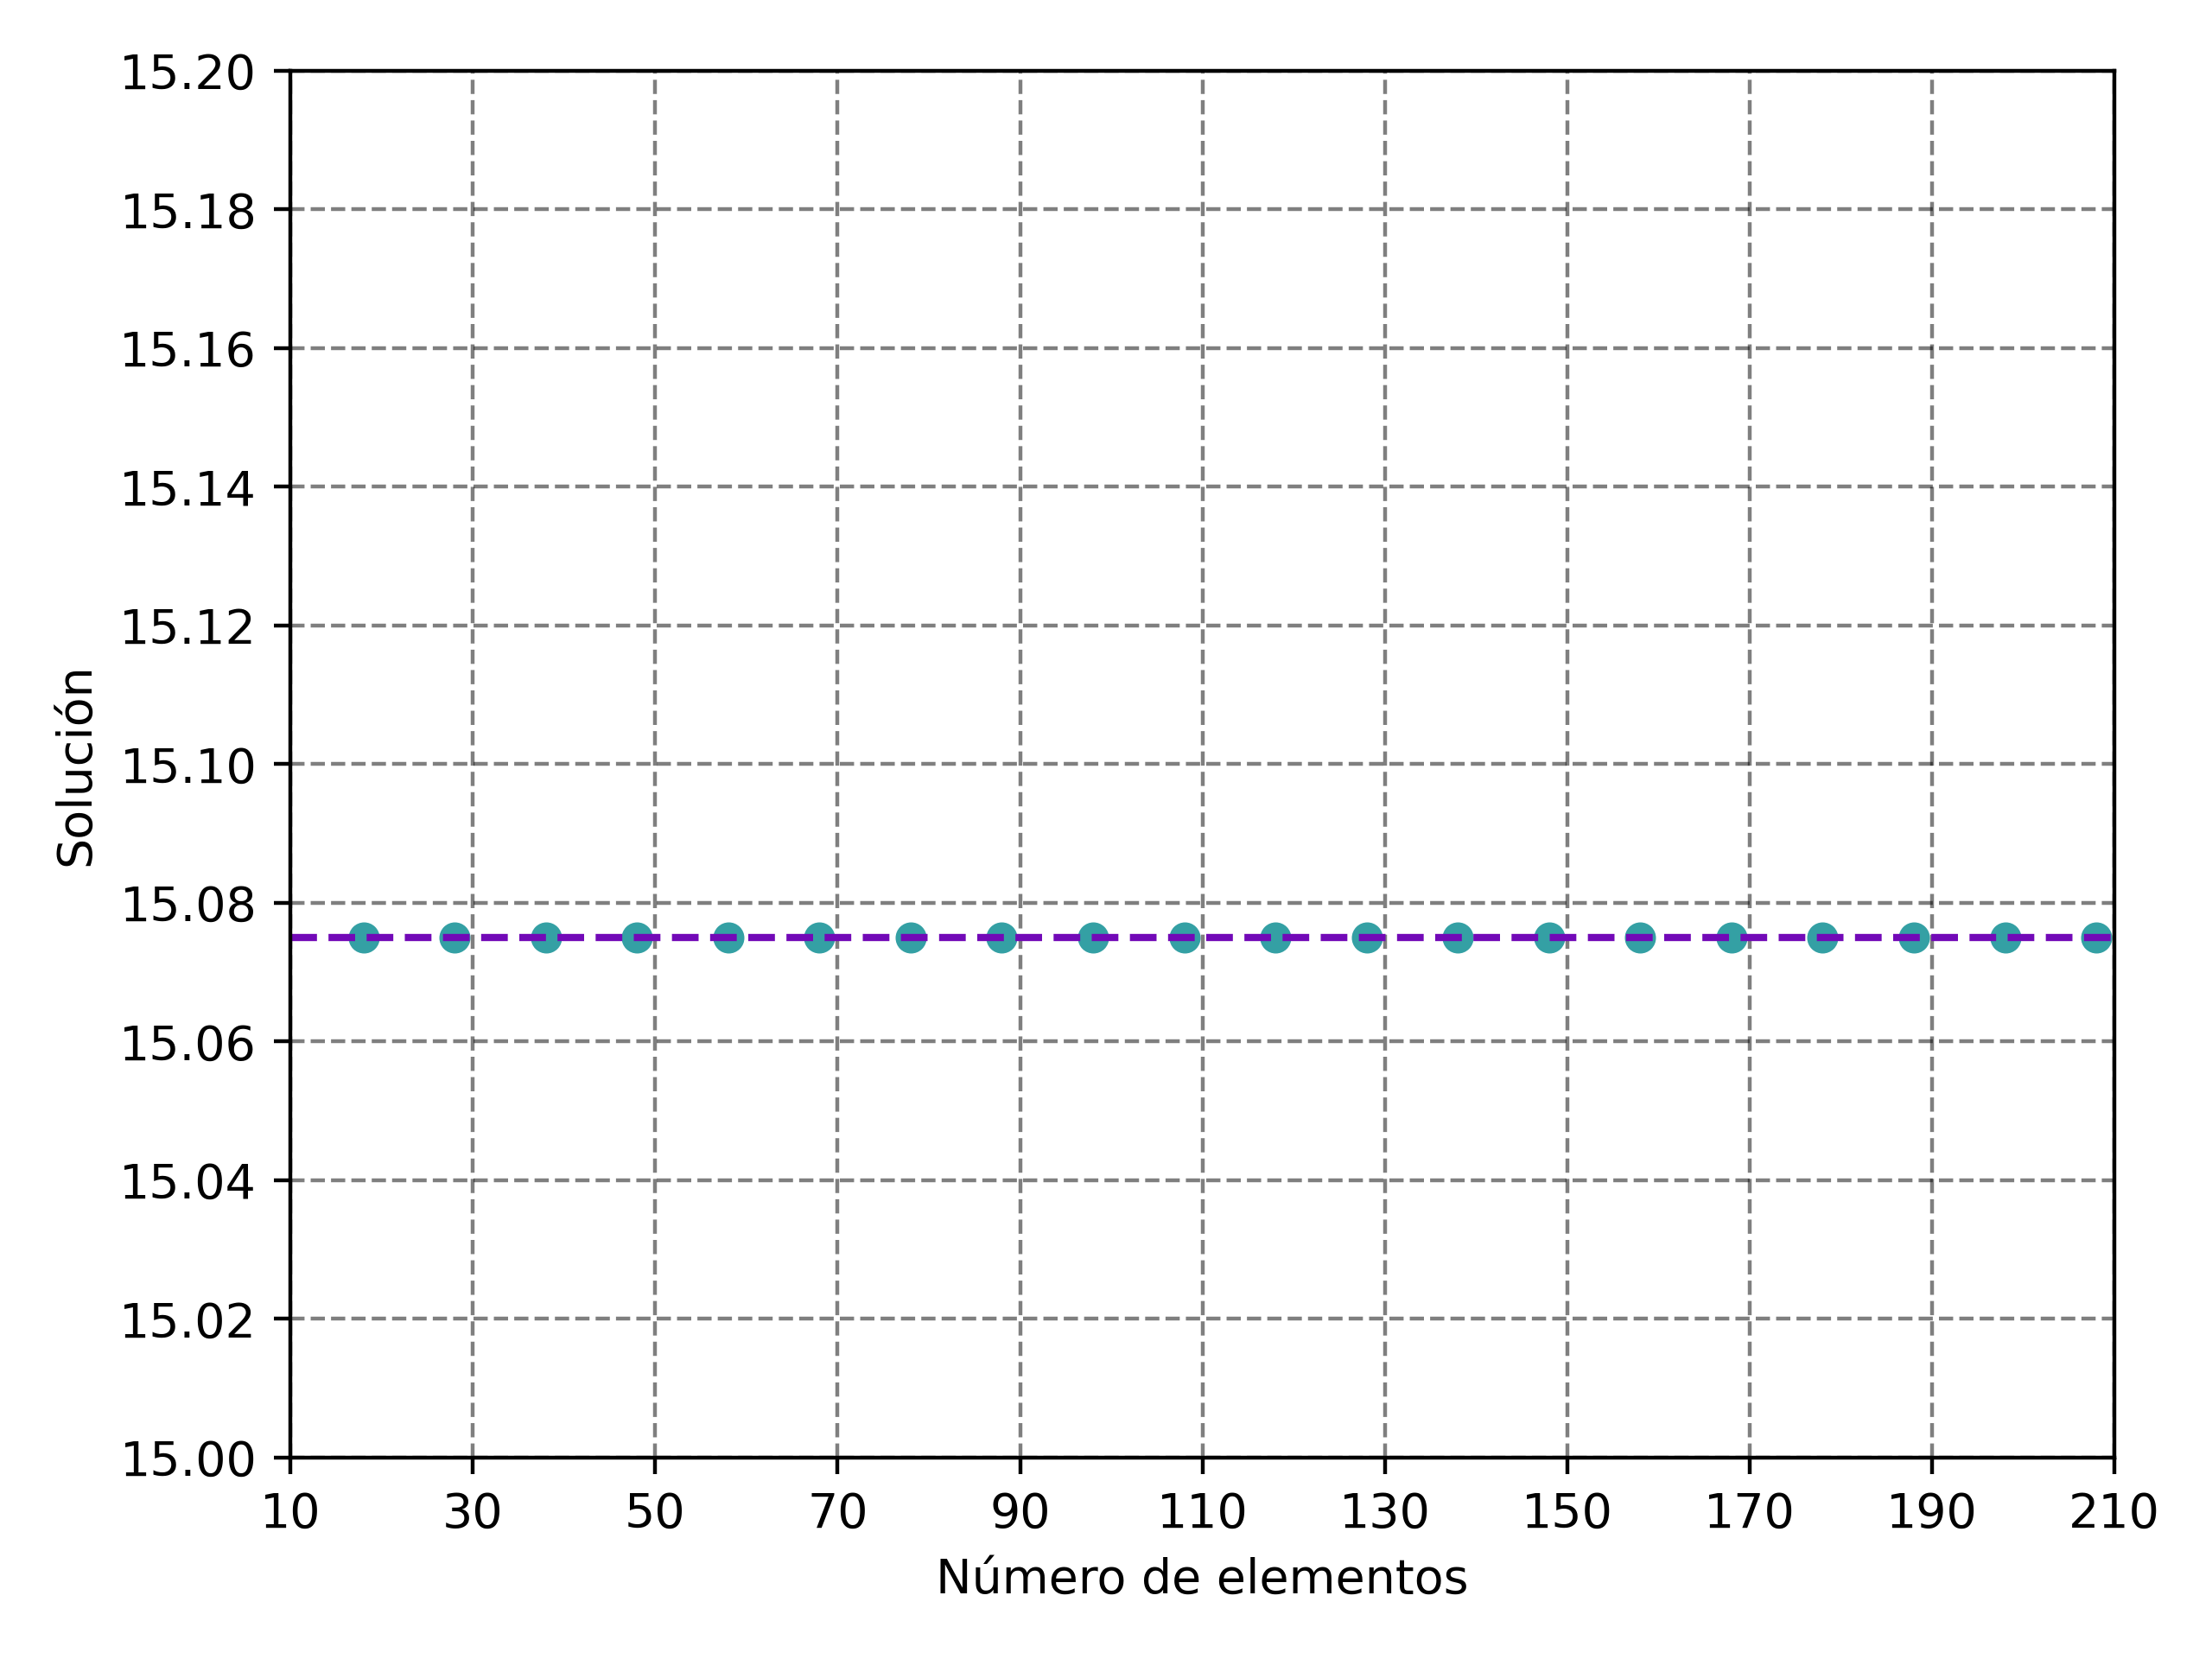
\includegraphics[width=7.5cm]{Graphics/heat_results_2.png}
            \caption{Resultado del nodo anterior al central ($\frac{n}{2}-1$) para cada valor de n.}
            \label{fig:heat_results_2}
        \end{figure}
    \end{minipage}
\end{center}